\documentclass[a4paper,10pt,oneside]{article}
\usepackage{graphicx}
\usepackage{color}
\usepackage{url}
\usepackage{subfigure}
\usepackage[utf8]{inputenc}
\usepackage[T1]{fontenc}
\usepackage{tgpagella}
%\usepackage[scale=0.9]{tgcursor}
%\usepackage[scale=0.9]{tgheros}
\usepackage{xstring}

\newcommand{\myscale}{0.74}
\newcommand{\vect}[1]{\boldsymbol{#1}}
\newcommand{\code}[1]{\texttt{\StrSubstitute{#1}{.}{.\.}}}
\def\.{\discretionary{}{}{}}
\newcommand{\jmodule}[1]{\texttt{\textit{#1}}}

\setlength{\hoffset}{-1in} %left margin will be 0, as hoffset is by default 1inch
\setlength{\voffset}{-1in} %analogous voffset
\setlength{\oddsidemargin}{1.5cm}
\setlength{\evensidemargin}{1.5cm}
\setlength{\topmargin}{1.5cm}
\setlength{\textheight}{24cm}
\setlength{\textwidth}{18cm}

\def\mftitle{jInfer ProjectType Module Description}
\def\mfauthor{Michal Klempa, Mário Mikula, Robert Smetana, Michal Švirec, Matej Vitásek}
\def\mfadvisor{RNDr. Irena Mlýnková, Ph.D., Martin Nečaský, Ph.D.}
\def\mfplacedate{Praha, 2011}
\title{\bf\mftitle}
\author{\mfauthor \\ Advisors: \mfadvisor}
\date{\mfplacedate}

\ifx\pdfoutput\undefined\relax\else\pdfinfo{ /Title (\mftitle) /Author (\mfauthor) /Creator (PDFLaTeX) } \fi

\begin{document}
\maketitle
\noindent Target audience: developers willing to extend jInfer, specifically extend jInfer project structure.

\noindent \begin{tabular}{|l|l|} \hline
Responsible developer: & Michal Švirec \\ \hline
Required tokens:       & cz.cuni.mff.ksi.jinfer.base.interfaces.inference.IGGenerator \\
 & cz.cuni.mff.ksi.jinfer.base.interfaces.inference.SchemaGenerator \\
 & cz.cuni.mff.ksi.jinfer.base.interfaces.inference.Simplifier \\
 & org.openide.windows.IOProvider \\ \hline
Provided tokens:       & none \\ \hline
Module dependencies:   & Base \\
	& Runner \\ \hline
Public packages:       & cz.cuni.mff.ksi.jinfer.projecttype.actions \\ \hline
\end{tabular}

\section{Introduction}

\jmodule{ProjectType} is the module responsible for creation of NBP project type which groups input/output files that belongs to one specific inference. Each jInfer project also allows user to set properties specific for inference.\\

\begin{figure}
	\centering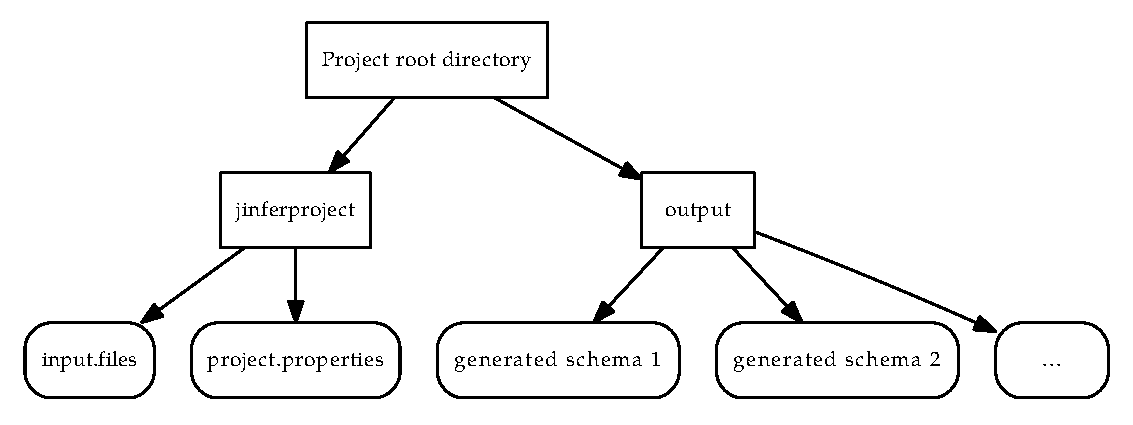
\includegraphics[scale=\myscale]{project_dir_structure}
	\caption{Project directory structure} \label{dir-structure}
\end{figure}

With each project created in jInfer is also created specific directory structure on filesystem that describes jInfer project. This structure is described in figure \ref{dir-structure}, where rectangles represent folders and rounded rectangles files. Folder in filesystem is considered as jInfer project folder, if contains \emph{jinferproject} subfolder. These folder contains two files, first is \emph{project.properties}, where all properties set for particular project are saved. Second file is \emph{input.files} which is xml file filled with paths to files inserted as input into particular project (structure of this file is described in section \ref{input.files}).

\section{Structure}

Structure of \jmodule{ProjectType} can be divided into following five main parts.
\begin{itemize}
	\item Base classes - Classes providing main functionality like creation of project, defining operations like move, delete, copy etc. All the base classes are contained in the \code{cz.cuni.mff.ksi.jinfer.projecttype} package.
	\item Visualization classes - These classes create tree structure of project in NBP Projects view and are contained in the \code{cz.cuni.mff.ksi.jinfer.projecttype.nodes}
	\item Actions - Classes from \code{cz.cuni.mff.ksi.jinfer.projecttype.actions} package that provides actions allowing adding, removing input files into project, or running the project.
	\item Properties - Classes responsible for creation of project properties window with properties category tree. These are situated in  \code{cz.cuni.mff.ksi.jinfer.projecttype.properties} package.
	\item Project wizard - Classes representing creation of project through new project wizard from  \code{cz.cuni.mff.ksi.jinfer.projecttype.sample} package.
\end{itemize}

\subsection{Base classes}


This section describes classes needed for creation of the jInfer project and correct integration into NBP. Main two classes representing jInfer project type are \code{JInferProjectFactory} and \code{JInferProject}.

\subsubsection{JInferProjectFactory}

\code{JInferProjectFactory} is a factory class implementing \code{ProjectFactory} interface provided by NBP. This class is responsible for loading/saving of jInfer project from/to filesystem and also determining if folder in filesystem is type of jInfer project (contains \emph{jinferproject} subfolder). For this purpose, class has three methods: \code{isProject()}, \code{save()} and \code{load()}. When jInfer project is loaded from filesystem, \code{JInferProjectFactory} creates new instance of \code{JInferProject} passing path to project folder as a constructor parameter. When \code{save()} method is invoced, all the project properties are saved in \emph{projectproperties} file and paths to input files are saved in \emph{input.files}.

\subsubsection{JInferProject}

\code{JinferProject} class implements \code{Project} interface from NBP and represents in-memory representation of jInfer project. Inner structure of this class is very simple, interface provides only two methods: \code{getProjectDirectory()} and \code{getLookup()}. All the extensibility of project type is done by \emph{Lookup} functionality of NBP. Project lookup contains besides properties and \code{Input} class, which encapsulates input files, also class that creates output files, class that builds project tree in project window, etc.

\subsubsection{InputFiles class}\label{input.files}

\code{InputFiles} is utility class that stores/loads input file paths into/from input.files xml file. For this purpose, class uses \emph{JAXB} architecture to unmarshall/marshall xml file into/from java content objects. Xml structure of the input.files is very simple, \emph{jinferinput} is root element under which are \emph{xml}, \emph{schemas} and \emph{queries} elements. Each of this elements could have none or more \emph{file} elements with string attribute \emph{loc} that contains absolute path to input file.\\

\noindent Example of the structure follows.
\begin{verbatim}
	<?xml version="1.0" encoding="UTF-8" standalone="yes"?>
	<jinferinput>
	    <xml>
	        <file loc="/home/user/example.xml"/>
	    </xml>
	    <schemas>
		<file loc="/home/user/example.dtd"/>
	    </schemas>
	    </queries/>
	</jinferinput>
\end{verbatim}

\subsection{Visualization classes}



\subsection{Actions}

\subsection{Properties}

\subsection{Project wizard}

\subsection{Preferences}


\nocite{*}
\newpage
\bibliographystyle{alpha}
\bibliography{literature}

\end{document}
